\section{Постановка задачи}

В домашней работе №1 численными методами решается задача теплопроводности вида:

\begin{equation}
\begin{array}{l}
\dfrac{\partial u}{\partial t} = \alpha \dfrac{\partial^2 u}{\partial x^2} + f(x, t), \; t > 0, \; x \in (0, l_x), \\
\left. u \right|_{t=0} = u_0(x), \\
\left. u \right|_{x=0} = \mu_1(t), \\
\left. u \right|_{x=l_x} = \mu_2(t),
\end{array}
\end{equation}

где $u(x, t)$ - функция температуры, $\alpha = const$ - коэффициент теплопроводности, $f(x, t)$ - функция источника. 

Задача решается двумя разностными методами - явным и неявным. 
Зададим дискретную по времени (с шагом $\tau$) и пространству (с шагом $h$) сетку состояний $u(x_i,t_k) = u(h*i, \tau*k) = y^k_i$
Так же в рамках задачи оценивается шкалирование ошибки обоих методов с реальным (аналитическим решением) относительно временного шага $\tau$ и пространственного $h$.

Эксперименты проводятся на следующих двух задачах:

\begin{equation}
\begin{cases}
\dfrac{\partial u}{\partial t} = \dfrac{\partial^2 u}{\partial x^2}, \; t > 0, \; x \in (0, 1), \\
\left. u \right|_{t=0} = 0, \\
\left. u \right|_{x=0} = 1, \\
\left. u \right|_{x=l_x} = 1,
\end{cases}
\label{eq:task1}
\end{equation}


\begin{equation}
\begin{cases}
\dfrac{\partial u}{\partial t} = \dfrac{\partial^2 u}{\partial x^2}, \; t > 0, \; x \in (0, \pi), \\
\left. u \right|_{t=0} = \sin{(4\pi)}, \\
\left. u \right|_{x=0} = 0, \\
\left. u \right|_{x=l_x} = 0,
\end{cases}
\label{eq:task2}
\end{equation}

Очевидно, что в отсутствии собственного источника ($f(t,x) = 0$) и константных краевых условиях, системы имеют предельное состояние:

\[\exists \lim\limits_{t \rightarrow \infty} u(x, t) = u_\infty (x).\]

В первом случае это - $u_{\infty1} (x) = 1$, во втором - $u_{\infty1} (x) = 0$. 
Поэтому обе схемы будут считаться до установления сходимости их состояний,
то есть пока вектор разницы состояний в смежные моменты времени не будет по модулю меньше заданного пользователем $\epsilon > 0$:

\[ ||u^{k+1} - u^k|| < \epsilon \]

Ошибка будет расчитываться для задачи \ref{eq:task2} - её аналитическое решение равно:

\[ u_2(x,t) = \sin{(4x)}\exp{(-16t)} \]

\newpage
\section{Явный метод}

Запишем разностное уравнение явной схемы:
$$\dfrac{y_i^{k+1} - y_i^{k}}{\tau} = \alpha \dfrac{y_{i+1}^{k} - 2 y_i^{k} + y_{i-1}^{k}}{h^2} + f_i^k,$$
где $\tau$ и $h$ - шаги по времени и пространству, $y_i^k$ - значение приближённого решения в точке $(i, k)$ сетки, $y_i^k$ - значение функции источника в той же точке сетки. 

Аппроксимируем начальное и граничные условия:
\begin{equation}
\begin{array}{l}
y_i^0 = u_0(x_i), \; \forall i = \overline{0, N},\\
y_0^k = \mu_1(t_k), \\
y_N^k = \mu_2(t_k), \; \forall k > 0.
y_i^k = y_i^{k-1} + \frac{\alpha \tau}{h^2} \left(y_{i+1}^{k-1} - 2 y_i^{k-1} + y_{i-1}^{k-1})
\end{array}
\end{equation}

Реализация кода явной схемы представлена в приложении \ref{expl}. Схема была проверена следующими тестами:

\begin{itemize}
\item Задача \ref{eq:task1}, $h=0.1, \tau=0.005, \epsilon=10^{-3}$. Решение должно отличаться от предельного не более чем на $10^{-2}$
\item Задача \ref{eq:task2}, $h=0.1, \tau=0.005, \epsilon=10^{-3}$. Решение должно отличаться от предельного не более чем на $10^{-2}$
\end{itemize}

Оба опыта оказались успешными. Далее необходимо оценить шкалирование одной из ошибок (была выбрана зависимость ошибки от пространственного шага):

Были взяты несколько значений шага $h = 0.05, 0.1, 0.2, 0.4$. На основании моментов сходимости результатов (моментов когда программа прекращала свой расчёт) в качестве измеряемого момента времени был выбран $t_1 = 0.15$. Графики сходимости ошибки между соседними слоями можно увидеть на картинке \ref{fig:expl_t1}.

\begin{figure}
\centering
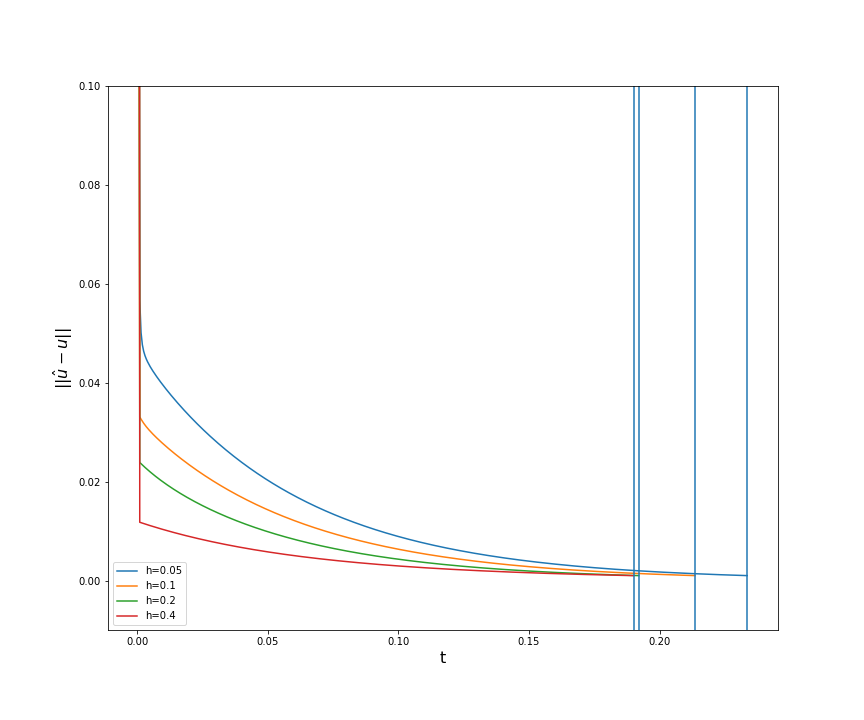
\includegraphics[width=0.7\textwidth]{expl_t1.png}
\caption{График сходимости состояния к предельному от времени по явной схеме}
\label{fig:expl_t1}
\end{figure} 

Теперь рассчитаем ошибку задачи для схем с шагами $h = 0.05, 0.1, 0.2, 0.4$ при $\tau=0.0005$ между вычисляемым и реальным значением в момент времени $t_1$ (cм. график \ref{fig:expl_err})

\begin{figure}
\centering
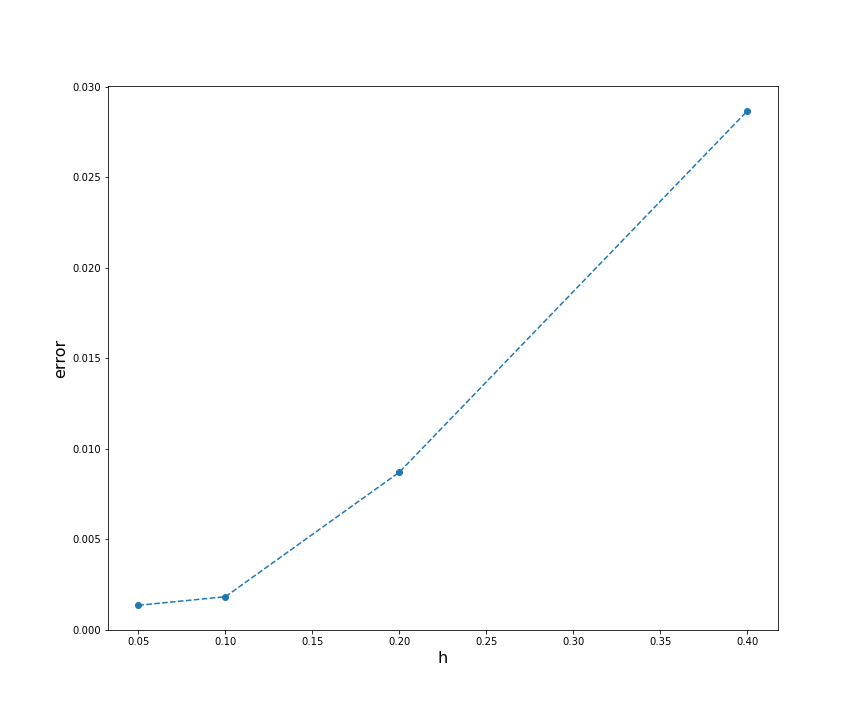
\includegraphics[width=0.7\textwidth]{expl_err.png}
\caption{График ошибки между численным состоянием и истинным (в тех же местах сетки) от длины шага сетки в пространстве по явной схеме}
\label{fig:expl_err}
\end{figure} 

График \ref{fig:expl_err} показывает квадратичный характер шкалирования ошибки (то есть, при увеличении шага в два раза, ошибка увеличивается почти в четыре).

\newpage
\section{Неявный метод}

Запишем разностное уравнение неявной схемы:
$$\dfrac{y_i^{k+1} - y_i^{k}}{\tau} = \alpha \dfrac{y_{i+1}^{k+1} - 2 y_i^{k+1} + y_{i-1}^{k+1}}{h^2} + f_i^{k+1}.$$

Поскольку в данном случае неизвестными в одном уравнения являются сразу три переменные ($y_{i+1}^{k+1}$, $y_i^{k+1}$и $y_{i-1}^{k+1}$), для нахождения значений следующего слоя необходимо решить систему из $N-2$ уравнений (краевые уравнения не считаются) вида:

\[ -D y_{i+1}^{k+1}  + (1 + 2 D)y_i^{k+1} - D y_{i-1}^{k+1} = y_i^k + f^{k+1}_i\]
\[ D =  \frac{\alpha \tau}{h^2} \]

Получим систему вида:

\begin{equation*}
 A = 
 \begin{pmatrix}
	1+2D & -D & 0 & \cdots & 0 \\
	-D & 1+2D & -D & \cdots & 0 \\
	0 &  & \cdots &  &  0 \\
	0 & \cdots & -D & 1+2D & -D \\
	0 & \cdots & 0 & -D & 1+2D\\
 \end{pmatrix},
 \ \ \ \ \ b = 
 \begin{pmatrix}
  y_1 + D y_0 \\
  y_2 \\
  \cdots \\
  y_{N-3} \\
  y_{N-2} + D y_{N-1} \\
 \end{pmatrix}
\end{equation*}

В случаях $i=1, N-2$ переменые $y_{i-1}^{k+1}$ и $y_{i+1}^{k+1}$ соответственно известны из краевых услових в переходят вправо как константы. Функция источника в наших задачах отсутствует.

Опыты, проделанные ранее с явной схемой оказались успешными так же и в неявной схеме. Далее перейдём к подбору измеряемого момента времени ($\tau=0.0005, h=0.0125, 0.025, 0.05, 0.1, 0.2, 0.4$ ). На основании графика ошибки между слоями получим, что на подходит $t_1=0.15$

\begin{figure}
\centering
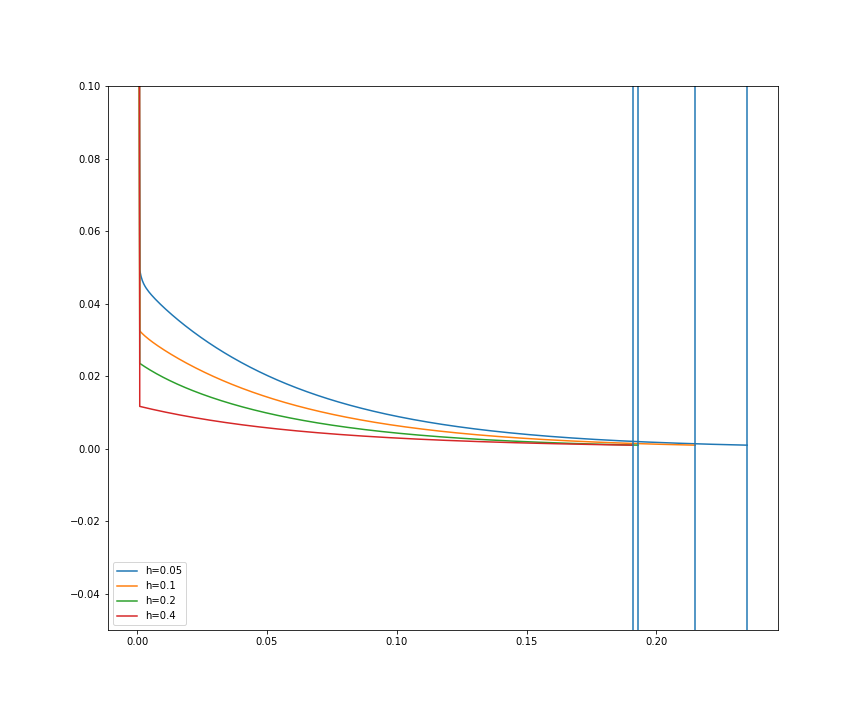
\includegraphics[width=0.7\textwidth]{impl_t1.png}
\caption{График сходимости состояния к предельному от времени по неявной схеме}
\label{fig:impl_t1}
\end{figure} 

\begin{figure}
\centering
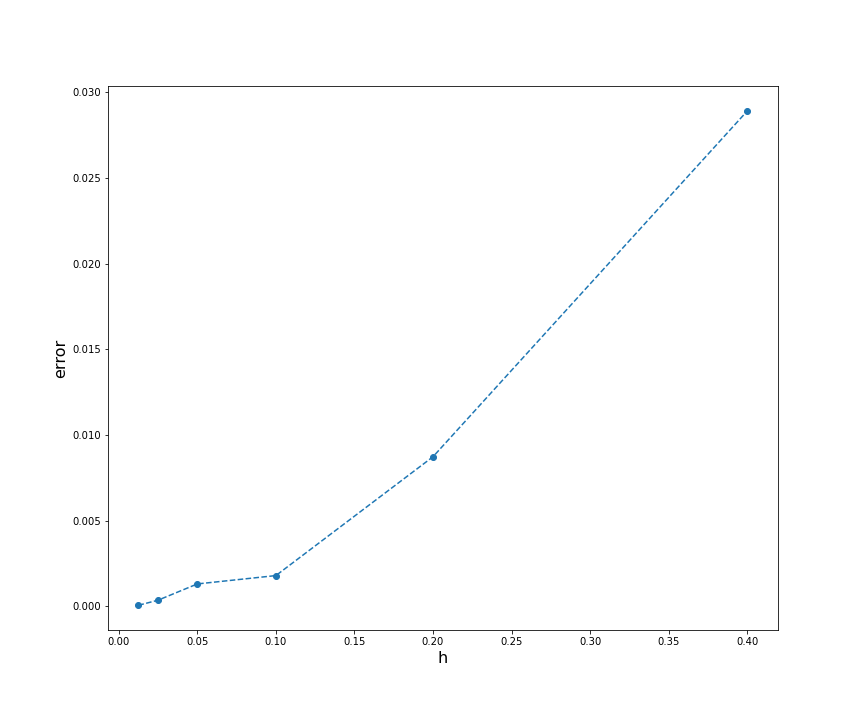
\includegraphics[width=0.7\textwidth]{impl_err.png}
\caption{График ошибки между численным состоянием и истинным (в тех же местах сетки) от длины шага сетки в пространстве по неявной схеме}
\label{fig:impl_err}
\end{figure} 

Точно так же как и в схеме явного метода, ошибка от пространственного шага шкалируется квадратично, как видно из графика \ref{fig:impl_err}.

\newpage

\section{Приложение}

\begin{lstlisting}[language=Python, caption=Реализация явного метода на языке Python, label=expl]
import numpy as np

def heat_expl(init, bound1, bound2, alpha, lx, h, tau, tol=1e-3):
    """ Solve the heat equation `u_t = a*u_xx` for x in (0; lx) with an explicit scheme.
    
    Parameters
    ----------
    init : callable
       Initial condition
    bound1 : callable
       Boundary condition for x = 0
    bound1 : callable
       Boundary condition for x = lx
    alpha : float
       Thermal diffusivity
    h : float
       Spatial step
    tau : float
       Time step
    tol : float, optional
       Target tolerance.
       Stop iterations when the 2-norm of the difference between 
       solution on this time step and the next is less the tol.
       
    Returns
    -------
    t_end : float
       End time of calculation
    u_end : ndarray, shape (N,)
       Limit u_∞(x) (See above)
    """
    
    # YOUR CODE HERE
    w_x = np.arange(0, lx+h, h)[:int(lx/h)+1]
    t_0 = 0.
    
    t_end = t_0 + tau
    u_0 = np.array([init(x) for x in w_x], dtype=np.float64)
    u_end = np.zeros(u_0.shape)
    
    u_end[0] = bound1(t_end)
    u_end[-1] = bound2(t_end)
    for i in range(1, len(u_end)-1):
        u_end[i] = u_0[i] + tau * alpha / (h ** 2) * (u_0[i+1] - 2 * u_0[i] + u_0[i-1])
    
    while np.linalg.norm(u_end - u_0) >= tol:
        u_0 = u_end.copy()
        t_end += tau
        u_end[0] = bound1(t_end)
        u_end[-1] = bound2(t_end)
        for i in range(1, len(u_end)-1):
            u_end[i] = u_0[i] + tau * alpha / (h ** 2) * (u_0[i+1] - 2 * u_0[i] + u_0[i-1])
    
    
    
    return t_end, u_end

\end{lstlisting}

\newpage

\begin{lstlisting}[language=Python, caption=Реализация неявного метода на языке Python]
import numpy as np
from scipy.linalg import solve_banded

def heat_impl(init, bound1, bound2, alpha, lx, h, tau, tol=1e-3):
    """ Solve heat equation u_t = a*u_xx for x in (0; lx) with implicit scheme
    
    Parameters
    ----------
    init : callable
       Initial condition
    bound1 : callable
       Boundary condition for x = 0
    bound1 : callable
       Boundary condition for x = lx
    alpha : float, optional
       Thermal diffusivity
    h : float
       Spatial step
    tau : float
       Time step
    tol : float, optional
       Target tolerance.
       Stop iterations when the 2-norm of the difference between 
       solution on this time step and the next is less the tol.
       
    Returns
    -------
    t_end : float
       End time of calculation
    u_end : ndarray, shape (N,)
       Limit u_∞(x) (See above)
    """
    
    w_x = np.arange(0, lx+h, h)[:int(lx/h)+1]
    t_0 = 0.
    t_end = t_0 + tau
    u_0 = np.array([init(x) for x in w_x], dtype=np.float64)
    N = u_0.shape[0]
    
    A = np.zeros((N-2,N-2), dtype=np.float64)
    b = np.zeros(N-2, dtype=np.float64)
    u_end = np.zeros(N, dtype=np.float64)
    u_end[0] = bound1(t_end)
    u_end[-1] = bound2(t_end)
    
    A[0][:2] = (2 * alpha * tau / np.power(h, 2) + 1), -(alpha * tau / np.power(h, 2))
    b[0] = u_0[1] + (alpha * tau / np.power(h, 2)) * u_end[0]
    for i in range(1,N-3):
        A[i][i-1], A[i][i], A[i][i+1] = -(alpha * tau / np.power(h, 2)), (2 * alpha * tau / np.power(h, 2) + 1), -(alpha * tau / np.power(h, 2))
        b[i] = u_0[i+1]
    A[-1][-2:] = -(alpha * tau / np.power(h, 2)), (2 * alpha * tau / np.power(h, 2) + 1)
    b[-1] = u_0[-2] + (alpha * tau / np.power(h, 2)) * u_end[-1]
    ab = np.zeros((3, A.shape[0]))
    ab[0,1:] = np.diag(A,k=1)
    ab[1] = np.diag(A)
    ab[2,:-1] = np.diag(A, k=-1)
    u_end[1:-1] = solve_banded((1,1),ab,b) 
    while np.linalg.norm(u_end - u_0) >= tol:
        u_0 = u_end.copy()
        t_end += tau
        
        u_end = np.zeros(N, dtype=np.float64)
        u_end[0] = bound1(t_end)
        u_end[-1] = bound2(t_end)
        
        b[0] = u_0[1] + (alpha * tau / np.power(h, 2)) * u_end[0]
        for i in range(1,N-3):
            b[i] = u_0[i+1]
        b[-1] = u_0[-2] + (alpha * tau / np.power(h, 2)) * u_end[-1]
        
        u_end[1:-1] = solve_banded((1,1),ab,b)   
        
    u_0 = u_end.copy()
    t_end += tau
    u_end = np.zeros(N, dtype=np.float64)
    u_end[0] = bound1(t_end)
    u_end[-1] = bound2(t_end)
    b[0] = u_0[1] + (alpha * tau / np.power(h, 2)) * u_end[0]
    for i in range(1,N-3):
        b[i] = u_0[i+1]
    b[-1] = u_0[-2] + (alpha * tau / np.power(h, 2)) * u_end[-1]
    u_end[1:-1] = solve_banded((1,1),ab,b) 
    
    return t_end, u_end
\end{lstlisting}
